\documentclass{standalone}
\usepackage{tikz}
\usetikzlibrary{patterns, positioning}


\begin{document}
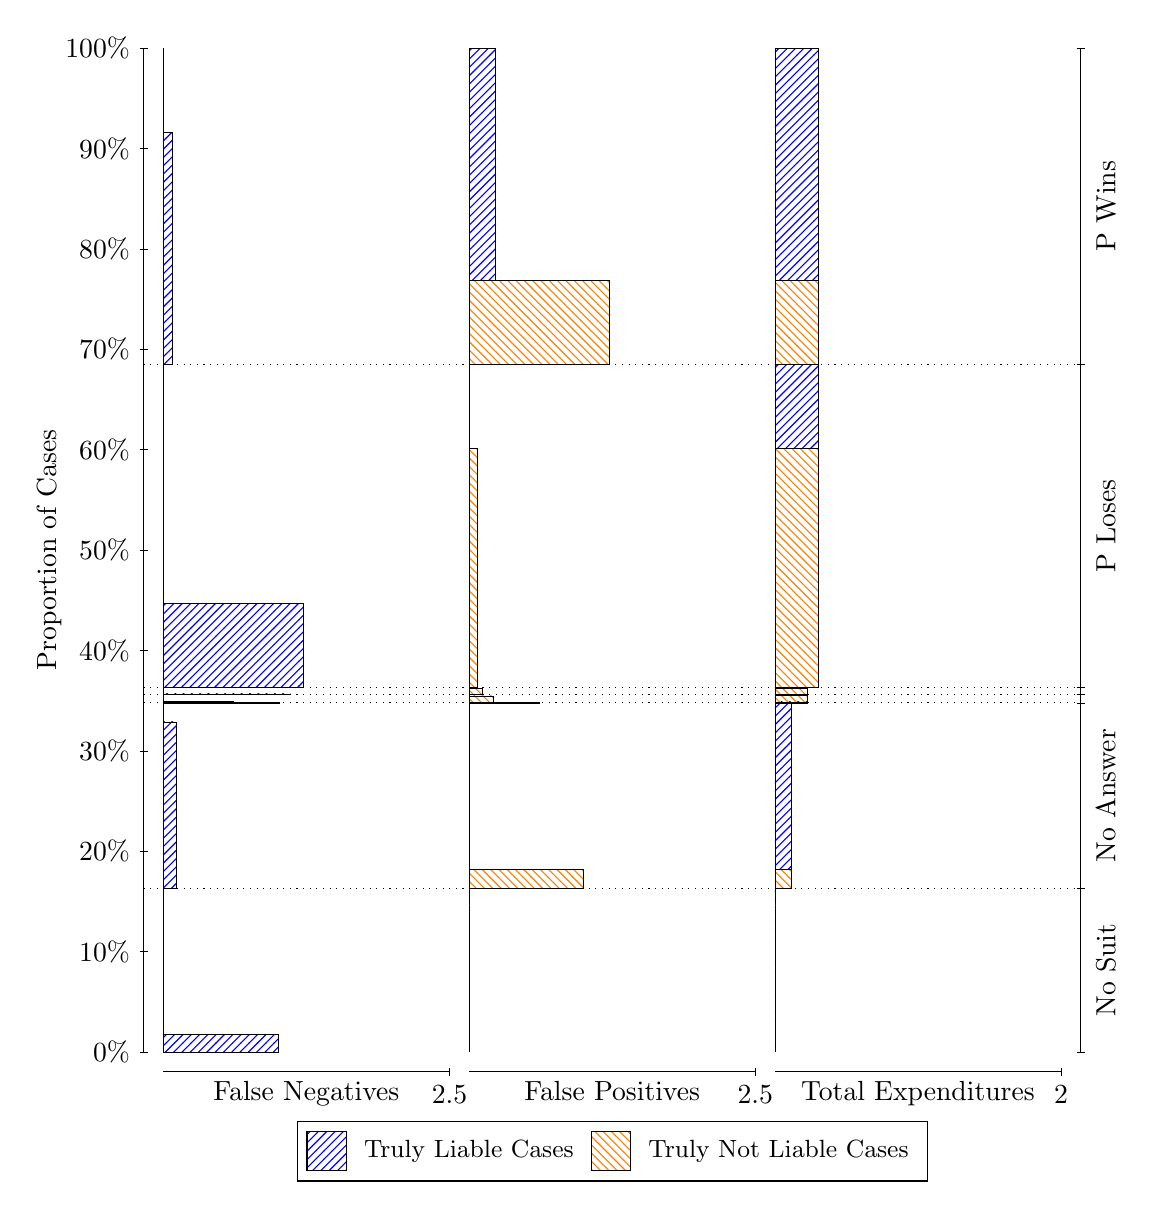
\begin{tikzpicture}
\draw[black, very thin] (1.5,1.75) -- (1.5,14.5);
\node[rotate=90, text=black, anchor=center] at (0.3, 8.125) {Proportion of Cases};
\draw[black, very thin] (1.45,1.75) -- (1.55,1.75);
\node[text=black, anchor=east] at (1.45, 1.75) {0\%};
\draw[black, very thin] (1.45,3.025) -- (1.55,3.025);
\node[text=black, anchor=east] at (1.45, 3.025) {10\%};
\draw[black, very thin] (1.45,4.3) -- (1.55,4.3);
\node[text=black, anchor=east] at (1.45, 4.3) {20\%};
\draw[black, very thin] (1.45,5.575) -- (1.55,5.575);
\node[text=black, anchor=east] at (1.45, 5.575) {30\%};
\draw[black, very thin] (1.45,6.85) -- (1.55,6.85);
\node[text=black, anchor=east] at (1.45, 6.85) {40\%};
\draw[black, very thin] (1.45,8.125) -- (1.55,8.125);
\node[text=black, anchor=east] at (1.45, 8.125) {50\%};
\draw[black, very thin] (1.45,9.4) -- (1.55,9.4);
\node[text=black, anchor=east] at (1.45, 9.4) {60\%};
\draw[black, very thin] (1.45,10.675) -- (1.55,10.675);
\node[text=black, anchor=east] at (1.45, 10.675) {70\%};
\draw[black, very thin] (1.45,11.95) -- (1.55,11.95);
\node[text=black, anchor=east] at (1.45, 11.95) {80\%};
\draw[black, very thin] (1.45,13.225) -- (1.55,13.225);
\node[text=black, anchor=east] at (1.45, 13.225) {90\%};
\draw[black, very thin] (1.45,14.5) -- (1.55,14.5);
\node[text=black, anchor=east] at (1.45, 14.5) {100\%};

\draw[black, very thin] (13.4,1.75) -- (13.4,14.5);
\draw[black, very thin] (13.35,1.75) -- (13.45,1.75);
\node[anchor=west] at (13.35, 1.75) {};
\draw[black, very thin] (13.35,3.8275) -- (13.45,3.8275);
\node[anchor=west] at (13.35, 3.8275) {};
\draw[black, very thin] (13.35,6.1847) -- (13.45,6.1847);
\node[anchor=west] at (13.35, 6.1847) {};
\draw[black, very thin] (13.35,6.287) -- (13.45,6.287);
\node[anchor=west] at (13.35, 6.287) {};
\draw[black, very thin] (13.35,6.3796) -- (13.45,6.3796);
\node[anchor=west] at (13.35, 6.3796) {};
\draw[black, very thin] (13.35,10.484) -- (13.45,10.484);
\node[anchor=west] at (13.35, 10.484) {};
\draw[black, very thin] (13.35,14.5) -- (13.45,14.5);
\node[anchor=west] at (13.35, 14.5) {};

\draw[black, very thin, pattern color=blue, pattern=north east lines] (1.75,1.75) rectangle (3.2033,1.9686);
\draw[black, very thin, pattern color=orange, pattern=north west lines] (1.75,1.9686) rectangle (1.75,3.8275);
\draw[black, very thin, pattern color=blue, pattern=north east lines] (1.75,3.8275) rectangle (1.9135,5.9427);
\draw[black, very thin, pattern color=orange, pattern=north west lines] (1.75,5.9427) rectangle (1.75,6.1847);
\draw[black, very thin, pattern color=blue, pattern=north east lines] (1.75,6.1847) rectangle (3.2215,6.1933);
\draw[black, very thin, pattern color=blue, pattern=north east lines] (1.75,6.1933) rectangle (3.0762,6.1938);
\draw[black, very thin, pattern color=blue, pattern=north east lines] (1.75,6.1938) rectangle (2.9308,6.1942);
\draw[black, very thin, pattern color=blue, pattern=north east lines] (1.75,6.1942) rectangle (2.7855,6.1943);
\draw[black, very thin, pattern color=blue, pattern=north east lines] (1.75,6.1943) rectangle (2.6402,6.1997);
\draw[black, very thin, pattern color=orange, pattern=north west lines] (1.75,6.1997) rectangle (1.75,6.287);
\draw[black, very thin, pattern color=blue, pattern=north east lines] (1.75,6.287) rectangle (3.3668,6.2964);
\draw[black, very thin, pattern color=orange, pattern=north west lines] (1.75,6.2964) rectangle (1.75,6.3796);
\draw[black, very thin, pattern color=blue, pattern=north east lines] (1.75,6.3796) rectangle (3.5303,7.4493);
\draw[black, very thin, pattern color=orange, pattern=north west lines] (1.75,7.4493) rectangle (1.75,10.484);
\draw[black, very thin, pattern color=blue, pattern=north east lines] (1.75,10.484) rectangle (1.859,13.431);
\draw[black, very thin, pattern color=orange, pattern=north west lines] (1.75,13.431) rectangle (1.75,14.5);
\draw[black, very thin, pattern color=orange, pattern=north west lines] (5.6333,1.75) rectangle (5.6333,3.6089);
\draw[black, very thin, pattern color=blue, pattern=north east lines] (5.6333,3.6089) rectangle (5.6333,3.8275);
\draw[black, very thin, pattern color=orange, pattern=north west lines] (5.6333,3.8275) rectangle (7.0867,4.0696);
\draw[black, very thin, pattern color=blue, pattern=north east lines] (5.6333,4.0696) rectangle (5.6333,6.1847);
\draw[black, very thin, pattern color=orange, pattern=north west lines] (5.6333,6.1847) rectangle (6.5235,6.1902);
\draw[black, very thin, pattern color=orange, pattern=north west lines] (5.6333,6.1902) rectangle (6.3782,6.1904);
\draw[black, very thin, pattern color=orange, pattern=north west lines] (5.6333,6.1904) rectangle (6.2328,6.1915);
\draw[black, very thin, pattern color=orange, pattern=north west lines] (5.6333,6.1915) rectangle (6.0875,6.1927);
\draw[black, very thin, pattern color=orange, pattern=north west lines] (5.6333,6.1927) rectangle (5.9422,6.2721);
\draw[black, very thin, pattern color=blue, pattern=north east lines] (5.6333,6.2721) rectangle (5.6333,6.287);
\draw[black, very thin, pattern color=orange, pattern=north west lines] (5.6333,6.287) rectangle (5.7968,6.3703);
\draw[black, very thin, pattern color=blue, pattern=north east lines] (5.6333,6.3703) rectangle (5.6333,6.3796);
\draw[black, very thin, pattern color=orange, pattern=north west lines] (5.6333,6.3796) rectangle (5.7423,9.4139);
\draw[black, very thin, pattern color=blue, pattern=north east lines] (5.6333,9.4139) rectangle (5.6333,10.484);
\draw[black, very thin, pattern color=orange, pattern=north west lines] (5.6333,10.484) rectangle (7.4137,11.553);
\draw[black, very thin, pattern color=blue, pattern=north east lines] (5.6333,11.553) rectangle (5.9603,14.5);
\draw[black, very thin, pattern color=orange, pattern=north west lines] (9.5167,1.75) rectangle (9.5167,3.6089);
\draw[black, very thin, pattern color=blue, pattern=north east lines] (9.5167,3.6089) rectangle (9.5167,3.8275);
\draw[black, very thin, pattern color=orange, pattern=north west lines] (9.5167,3.8275) rectangle (9.721,4.0696);
\draw[black, very thin, pattern color=blue, pattern=north east lines] (9.5167,4.0696) rectangle (9.721,6.1847);
\draw[black, very thin, pattern color=orange, pattern=north west lines] (9.5167,6.1847) rectangle (9.9254,6.1902);
\draw[black, very thin, pattern color=blue, pattern=north east lines] (9.5167,6.1902) rectangle (9.9254,6.1955);
\draw[black, very thin, pattern color=orange, pattern=north west lines] (9.5167,6.1955) rectangle (9.9254,6.2772);
\draw[black, very thin, pattern color=blue, pattern=north east lines] (9.5167,6.2772) rectangle (9.9254,6.2867);
\draw[black, very thin, pattern color=orange, pattern=north west lines] (9.5167,6.2867) rectangle (9.9254,6.2869);
\draw[black, very thin, pattern color=blue, pattern=north east lines] (9.5167,6.2869) rectangle (9.9254,6.287);
\draw[black, very thin, pattern color=orange, pattern=north west lines] (9.5167,6.287) rectangle (9.9254,6.3703);
\draw[black, very thin, pattern color=blue, pattern=north east lines] (9.5167,6.3703) rectangle (9.9254,6.3796);
\draw[black, very thin, pattern color=orange, pattern=north west lines] (9.5167,6.3796) rectangle (10.062,9.4139);
\draw[black, very thin, pattern color=blue, pattern=north east lines] (9.5167,9.4139) rectangle (10.062,10.484);
\draw[black, very thin, pattern color=orange, pattern=north west lines] (9.5167,10.484) rectangle (10.062,11.553);
\draw[black, very thin, pattern color=blue, pattern=north east lines] (9.5167,11.553) rectangle (10.062,14.5);
\draw[black, dotted] (1.5,3.8275) -- (13.4,3.8275);
\draw[black, dotted] (1.5,6.1847) -- (13.4,6.1847);
\draw[black, dotted] (1.5,6.287) -- (13.4,6.287);
\draw[black, dotted] (1.5,6.3796) -- (13.4,6.3796);
\draw[black, dotted] (1.5,10.484) -- (13.4,10.484);
\draw[black, very thin] (1.75,1.5) -- (5.3833,1.5);
\node[text=black, anchor=north] at (3.5667, 1.5) {False Negatives};
\draw[black, very thin] (5.3833,1.45) -- (5.3833,1.55);
\node[text=black, anchor=north] at (5.3833, 1.45) {2.5};

\draw[black, very thin] (5.6333,1.5) -- (9.2667,1.5);
\node[text=black, anchor=north] at (7.45, 1.5) {False Positives};
\draw[black, very thin] (9.2667,1.45) -- (9.2667,1.55);
\node[text=black, anchor=north] at (9.2667, 1.45) {2.5};

\draw[black, very thin] (9.5167,1.5) -- (13.15,1.5);
\node[text=black, anchor=north] at (11.333, 1.5) {Total Expenditures};
\draw[black, very thin] (13.15,1.45) -- (13.15,1.55);
\node[text=black, anchor=north] at (13.15, 1.45) {2};

\node[text=black, centered, rotate=90] at (13.72, 2.7888) {No Suit};
\node[text=black, centered, rotate=90] at (13.72, 5.0061) {No Answer};


\node[text=black, centered, rotate=90] at (13.72, 8.4316) {P Loses};
\node[text=black, centered, rotate=90] at (13.72, 12.492) {P Wins};

\draw (7.449999999999999,1.5) node[draw=none] (baseCoordinate) {};
\begin{scope}[align=center]
        \matrix[scale=0.5, draw=black, below=0.5cm of baseCoordinate, nodes={draw}, column sep=0.1cm]{
            \node[rectangle, draw, minimum width=0.5cm, minimum height=0.5cm, pattern color=blue, pattern=north east lines] {}; &
            \node[draw=none, font=\small, text=black] (B) {Truly Liable Cases}; &
            \node[rectangle, draw, minimum width=0.5cm, minimum height=0.5cm, pattern color=orange, pattern=north west lines] {}; &
            \node[draw=none, font=\small, text=black] (B) {Truly Not Liable Cases}; \\
            };
\end{scope}

\end{tikzpicture}
\end{document}